\documentclass{svproc}
%
% RECOMMENDED %%%%%%%%%%%%%%%%%%%%%%%%%%%%%%%%%%%%%%%%%%%%%%%%%%%
%

% to typeset URLs, URIs, and DOIs
\usepackage{url}
\usepackage{amsmath}
\usepackage{algorithm}
\usepackage[noend]{algpseudocode}

\usepackage{graphicx}
\usepackage{hyperref}

\usepackage{siunitx}
\usepackage{amsmath}
\usepackage{tikz}
\usepackage{adjustbox}
\usepackage{upgreek}
\usepackage{xcolor}
\usetikzlibrary{arrows, arrows.meta, fit, positioning, quotes,shadows, shapes.geometric, shapes.misc}
\usepackage[utf8]{inputenc}
\inputencoding{utf8}

\def\UrlFont{\rmfamily}

%%%%%%%%%%%%% math stuff
\usepackage{amssymb}

%flowchart definitions
\tikzstyle{startstop} = [rectangle, rounded corners, minimum width=3cm, minimum height=1cm,text centered, draw=black, fill=red!30]
\tikzstyle{io} = [trapezium, trapezium left angle=70, trapezium right angle=110, minimum width=3cm, minimum height=1cm, text centered, draw=black, fill=blue!30]
\tikzstyle{process} = [rectangle, minimum width=1cm, minimum height=1cm, text centered, draw=black, fill=white!30]
\tikzstyle{decision} = [diamond, minimum width=1cm, minimum height=1cm, text centered, draw=black, fill=cyan!30]
\tikzstyle{arrow} = [thick,->,>=stealth]

\tikzset{
  font={\fontsize{11pt}{12}\selectfont}}


% vectors in bold
\newcommand{\vp}{\mathbf{p}}
\newcommand{\valpha}{\mathbf{\alpha}}
\newcommand{\vP}{\mathbf{P}}
\newcommand{\vg}{\mathbf{g}}
\newcommand{\vf}{\mathbf{f}}
\newcommand{\vw}{\mathbf{w}}
\newcommand{\vx}{\mathbf{x}}
\newcommand{\vq}{\mathbf{q}}
\newcommand{\vzero}{\mathbf{0}}
\newcommand{\vn}{\mathbf{n}}
\newcommand{\vo}{\mathbf{o}}
\newcommand{\vchi}{\mathbf{\chi}}
\newcommand{\vlbA}{\mathbf{lbA}}
\newcommand{\vubA}{\mathbf{ubA}}
\newcommand{\vlb}{\mathbf{lb}}
\newcommand{\vub}{\mathbf{ub}}

% sets as caligraphics
\newcommand{\cV}{\mathcal{V}}
\newcommand{\cS}{\mathcal{S}}
\newcommand{\cC}{\mathcal{C}}
\newcommand{\cE}{\mathcal{E}}
\newcommand{\cO}{\mathcal{O}}
\newcommand{\cH}{\mathcal{H}}

% misc
\newcommand{\R}{\mathbb{R}} % real numbers
\renewcommand{\th}{^{\text{th}}}

\begin{document}
\mainmatter              % start of a contribution
\title{Robust Trajectory Execution for Multi-Robot Teams Using Distributed Real-time Replanning}
\titlerunning{Robust Trajectory Execution for Multi-Robot Teams}  % abbreviated title (for running head)
%                                     also used for the TOC unless
%                                     \toctitle is used
%
\author{Baskın Şenbaşlar \and Wolfgang H\"onig \and
Nora Ayanian}
%
%\authorrunning{Ivar Ekeland et al.} % abbreviated author list (for running head)
%
%%%% list of authors for the TOC (use if author list has to be modified)
\tocauthor{Baskın Şenbaşlar, Wolfgang H\"onig, Nora Ayanian}
%
\institute{University of Southern California, Los Angeles CA, USA,\\
\email{\{baskin.senbaslar, whoenig, ayanian\}@usc.edu}}

\maketitle              % typeset the title of the contribution

\begin{abstract}
Robust trajectory execution is an extension of cooperative collision avoidance that takes pre-planned trajectories directly into account.
We propose an algorithm for robust trajectory execution that compensates for a variety of dynamic changes, including newly appearing obstacles, robots breaking down, imperfect motion execution, and external disturbances.
Robots do not communicate with each other and only sense other robots' positions and the obstacles around them.
At the high-level we use a hybrid planning strategy employing both discrete planning and trajectory optimization with a dynamic receding horizon approach.
The discrete planner helps to avoid local minima, adjusts the planning horizon, and provides good initial guesses for the optimization stage.
Trajectory optimization uses a quadratic programming formulation, where all safety-critical parts are formulated as hard constraints.
At the low-level, we use buffered Voronoi cells as a multi-robot collision avoidance strategy.
Compared to ORCA, our approach supports higher-order dynamic limits and avoids deadlocks better.
We demonstrate our approach in simulation and on physical robots, showing that it can operate in real time.
%\keywords{trajectory planning, collision avoidance, multi-robot systems}
\end{abstract}


\section{Introduction}
Motion planning for multi-robot systems is particularly important in cases where many robots must interact with each other in confined spaces, potentially with many obstacles.
Examples include coordination of robots in warehouses~\cite{Kiva}, traffic management at intersections~\cite{IntersectionManagementDresner}, and airport management~\cite{AirportTug}.
Modern planning algorithms can find trajectories that effectively coordinate hundreds of robots while approximately optimizing objectives such as total energy used~\cite{crazyplanning-ieeetro};
however, all such solutions assume that the resulting trajectories can be executed nearly perfectly, which is an unrealistic assumption for teams of hundreds of robots that must operate persistently.

To compensate for changes in the environment or imperfect execution, one might apply cooperative collision avoidance strategies, such as ORCA~\cite{orca}, at runtime.
However, such algorithms often operate locally and do not take the pre-planned trajectories into account.
Robust trajectory execution, on the other hand, avoids future collision more effectively because it directly considers pre-planned trajectories.
Consider the example in Fig.~\ref{fig:swap2}(a), where two robots must swap positions.
The pre-planned trajectories are collision-free, but they do not consider the newly introduced obstacle and the blue robot does not start at its correct location.
However, the pre-planned trajectories can be used as guidance for replanning.
In this example, robots can get stuck if a local cooperative collision avoidance strategy is applied.
Using our method, the robots can successfully swap positions, while staying as close as possible to the pre-planned trajectories, as in Fig.~\ref{fig:swap2}(b).
Our method is fully distributed and requires no communication. The robots only need to know their own trajectories and be able to sense other robots' positions and the obstacles around them.

\begin{figure}
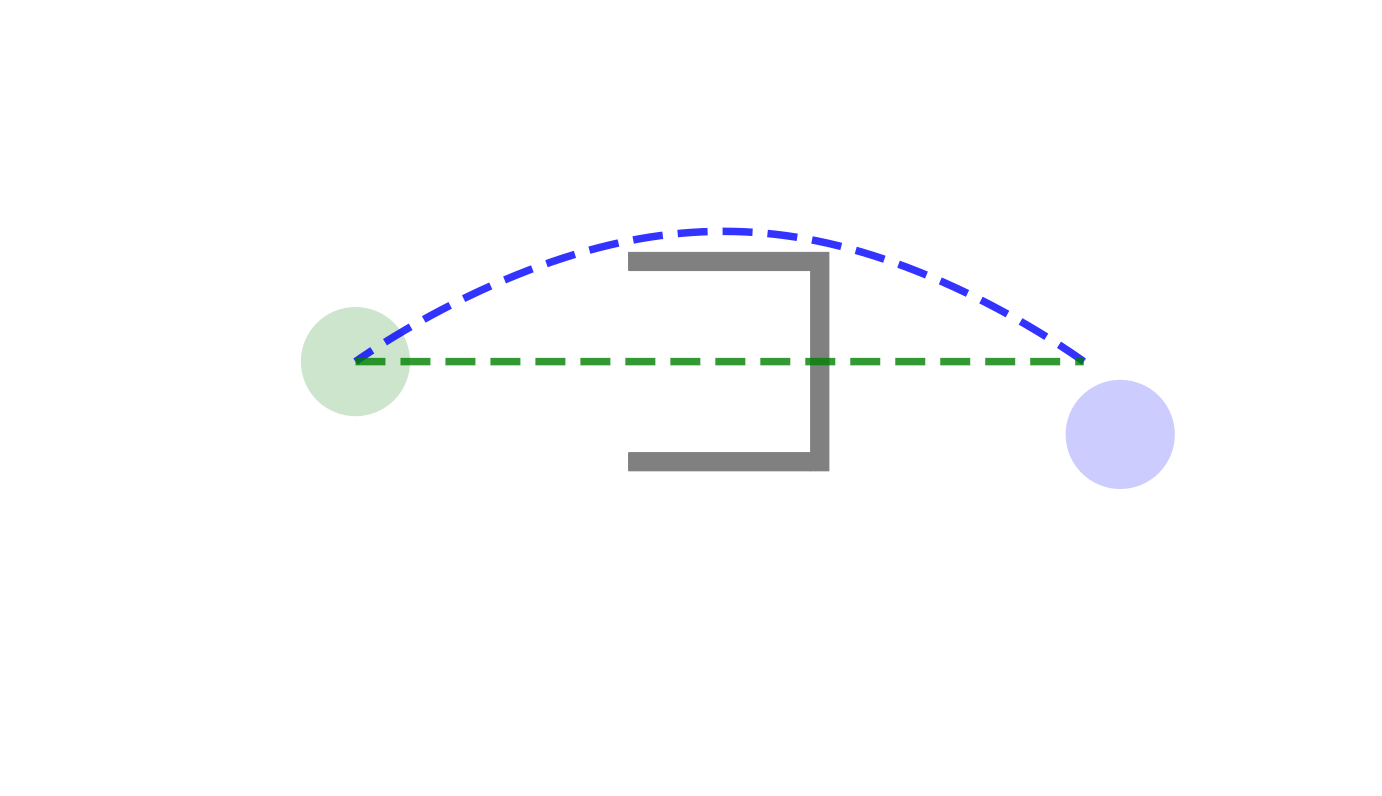
\includegraphics[width=0.45\textwidth]{images/swap2_initial.pdf}
\hfill
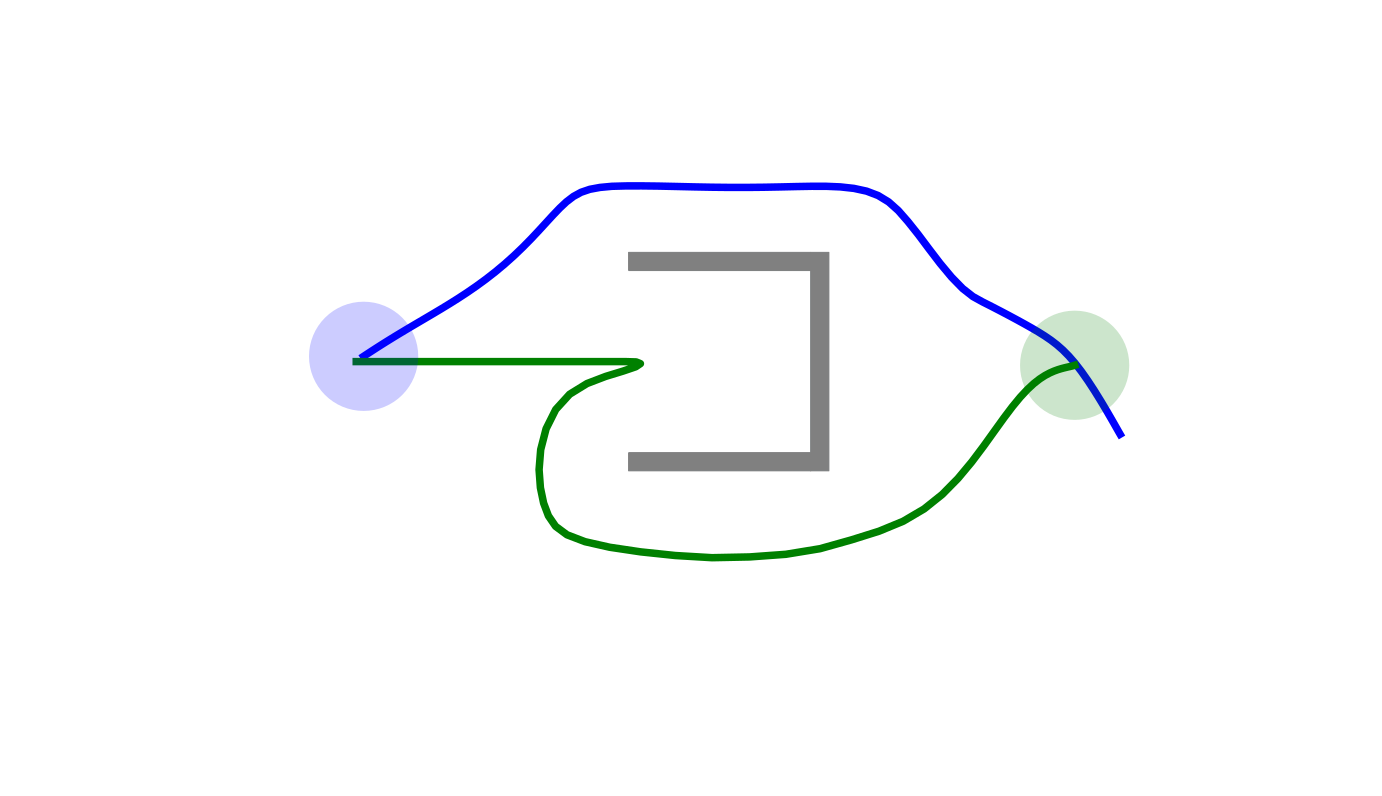
\includegraphics[width=0.45\textwidth]{images/swap2_final.pdf}
\caption{(a) Two robots (green and blue circles) are tasked with following their pre-planned trajectories (green and blue dashed lines).
The initial plans were created without the knowledge of the obstacle (gray) and the blue robot does not start at its planned initial position.
(b) Our approach computes smooth trajectories in real-time, avoiding both the new obstacle and other robots while staying close to the pre-planned trajectory.
}
\label{fig:swap2}
\end{figure}

Robust trajectory execution is an extension of cooperative collision avoidance where the objective is to stay as close to the originally planned trajectories as possible.
In contrast, traditional collision avoidance methods frequently only take a desired velocity, desired goal state, or desired action as input (we discuss these in more detail in Section~\ref{sec:relatedWork}).
Our method relies on \emph{Buffered Voronoi Cells} (BVC)~\cite{bufferedVoronoiCells} as the underlying cooperative collision avoidance strategy and retains the same theoretical guarantees.
We employ a novel combination of trajectory optimization and discrete search-based planning using a dynamic receding horizon approach.
The discrete search allows us to avoid local minima effectively even in difficult scenarios, while the trajectory optimization generates smooth trajectories that are collision-free.

The main contribution of this work is a novel distributed algorithm for robust trajectory execution that considers higher-order dynamic limits.
It also compensates for a variety of dynamic changes, including imperfect motion execution of robots, newly appearing obstacles, robots breaking down, or external disturbances.
We show in simulations that our method avoids deadlocks better than ORCA~\cite{orca}.
Furthermore, we implement and test our approach on a team of six differential drive robots with several dynamic environmental changes.

\section{Related Work}
\label{sec:relatedWork}
Our method is closely related to cooperative collision avoidance such as reciprocal velocity obstacles, buffered Voronoi cells, and safety barrier certificates.
Methods based on reciprocal velocity obstacles (RVO)~\cite{RVO} assume that robots continue with constant velocity and compute the safe configuration space such that no other robot might collide for the time horizon.
Many extensions of the RVO method have been proposed, see \cite{epsilonCCA} for an extensive overview.
Buffered Voronoi Cells (BVC)~\cite{bufferedVoronoiCells} compute the safe configuration space for a robot by its Voronoi cell shifted by the physical extent of the robot. 
Safety barrier certificates achieve collision-free operation by modifying a user-specified controller such that no collision can occur~\cite{barrierCertificates}.
Our robust trajectory execution approach uses cooperative collision avoidance at its core (specifically BVC), while extending it to minimize the difference to the original trajectories (rather than just a preferred velocity as in \cite{epsilonCCA}, preferred control input as in \cite{barrierCertificates}, or difference over a fixed time horizon as in \cite{bufferedVoronoiCells}.)

Our method is inspired by our previous work on offline planning for robotic teams~\cite{crazyplanning-ieeetro} and uses the same optimization framework based on B\'ezier curves to generate trajectories, although with a different cost function.
Similar to previous work we use discrete search to quickly get out of local minima, but do so in a distributed manner.

While our approach naturally works in multi-robot settings, some of the methods are inspired by single-robot optimization and collision avoidance.
Local collision avoidance for single robots such as UAVs can be formulated as optimization problems~\cite{replanning-eth,replanning-usenko}.
In both cases collisions are considered as a soft constraint in the cost function using a Euclidean (Signed) Distance Field.
In contrast, our formulation uses a hard constraint allowing us to easily detect infeasible trajectories.
The optimization can use a discrete plan as an initial guess~\cite{replanning-eth} or shift the existing trajectory based on newly appearing obstacles~\cite{replanning-usenko}.
In contrast, our approach shifts the existing trajectory whenever possible, while falling back to an efficient discrete planner with dynamic receding horizon to avoid local minima.

\section{Problem Formulation} \label{problemFormulation}
The general problem we would like to solve can be formulated as follows. 
Consider a group of $m$ robots. Each robot $i$ is given the following:
\begin{align*}
    \vo_i(t)&:\text{ original trajectory $(\R\to \R^n)$ of $i\th$ robot where time } t\in[0,T_i],\\
    c&:\text{ order of derivative up to which smoothness is required},\\
    R(\vp)&:\text{ convex collision shape of any robot at position $\vp$},\\
    \gamma_k&: \text{ dynamic limit of the robot for the $k\th$ derivative of its trajectory}.
\end{align*}

Each robot $i$ can sense the positions $\{\vp_1,\ldots,\vp_m\}$ of other robots as well as the current occupied space $\cO_i$ around it\footnote{Since our approach can accommodate many sensing modalities, we do not provide a specific sensing capability in the general problem.}.
We represent $\cO_i$ as a set of $\uptheta$ convex obstacles.
Robots are unaware of the other robots' planned trajectories, and cannot communicate with each other.
Each robot $i$ must execute a trajectory $\vf_i(t)$, where $\vf_i(t)$ is a solution to the following optimization problem:
\begin{align}
\begin{split}
    \text{minimize } & \int_{0}^{T_i}\left\|\vf_i(t)-\vo_i(t)\right\|^2 dt\\
    \text{subject to }& \\
    &\vf_i(t) \text{ is}\text{ continuous up to degree $c$},\\
    &\frac{d^j\vf_i}{dt^j}(0) = \frac{d^j\vp_i}{dt^j}(0)\text{ for } j\in\{0,1,...,c\}\\
    &\vf_i(t)\text{ is collision-free, and}\\ 
    &\left\|\frac{d^k \vf_i(t)}{dt^k}\right\| \leq \gamma_k\text{ for all desired $k$},\\
    \text{where } & t\in [0,T_i].
\end{split}
\label{eq:problem:opt}
\end{align}

We solve this problem approximately, using a dynamic receding horizon approach iteratively.
At every iteration $K$, robot $i$ plans a trajectory $\vf^{K}_i(t)$ that starts at the robots' current position and is safe to execute up to the user-provided period $\delta t$.
We set $R(\vp)$ to a sphere with radius $r_s$ centered at $\vp$.

\section{Preliminaries}
This section introduces important mathematical concepts and notations that will be used throughout the paper.

\subsection{Buffered Voronoi Cell} \label{bufferedVoronoi}
Given a set of $m$ robots with positions $\vp_1,\vp_2,\ldots,\vp_m \in \R^n$ and radii $r_s \in \R$, the buffered Voronoi cell $\cV_i$ of robot $i$ is defined as~\cite{bufferedVoronoiCells}:
\begin{align}
    \cV_i &= \left\{\vp : \forall_{j\neq i} \frac{\vp_j-\vp_i}{\|\vp_j-\vp_i\|}\cdot \vp - \frac{\vp_j-\vp_i}{\|\vp_j-\vp_i\|}\cdot \frac{\vp_j+\vp_i}{2} + r_s\leq 0 \right\}, \label{voronoi_cell_definition}
\end{align}
where $\|\vp\|$ is the L$^{2}$-norm of the vector $\vp$.

The inequality inside \eqref{voronoi_cell_definition} defines a hyperspace $\cS_i^j$ bounded by hyperplane $\cH_i^j$ that separates point $\vp_i$ from $\vp_j$. $\cH_i^j$ has normal $\valpha_i^j \in \R^n$ and distance $\beta_i^j\in \R$ along $\valpha_i^j$ such that
\begin{equation}
    \valpha_i^j = \frac{\vp_j - \vp_i}{\|\vp_j-\vp_i\|} \text{ and }
    \beta_i^j = \valpha_i^j \cdot \left(\frac{\vp_i + \vp_j}{2}\right) - r_s.
    \label{voronoiAlphaBeta}
\end{equation}

For a given buffered Voronoi decomposition of the space, any point $\vp\in \R^n$ can be inside of at most one of the buffered Voronoi cells.
We use this property in order to avoid robot-to-robot collisions.

Using the hyperspaces $\cS_i^j$ we can reformulate $\cV_i$ as follows:
\begin{equation}
    \cV_i = \bigcap\limits_{j\neq i} \cS_i^j \text{ , where } \cS_i^j = \left\{\vp : \valpha_i^j \cdot \vp - \beta_i^j \leq 0\right\}.
    \label{voronoiEquation}
\end{equation}

Thus, we can compute the buffered Voronoi cell of any robot $i$ as the set of the hyperplanes $\cH_i^j$ in $O(m)$ time.

\subsection{B\'ezier Curve} \label{bezierCurves}
A degree $d$ B\'ezier curve $\vf(t)$ implicitly parametrized by duration $T$ is defined by $d+1$ control points $\vP_0, \vP_1, ..., \vP_d \in \R^n$ such that
\begin{align}
    \vf(t) = \sum_{i=0}^d \vP_i {d\choose i}\left(\frac{t}{T}\right)^i\left(1-\frac{t}{T}\right)^{d-i},\hskip .5cm 0\leq t \leq T.
\end{align}

The curve starts at $\vP_0$ and ends at $\vP_d$, however does not interpolate other control points.
A B\'ezier curve lies completely inside the convex hull of its control points~\cite{Bernstein};
we leverage this property to avoid robot-to-obstacle collisions.

We use splines as trajectories with user-specified number of pieces ($l$) and degree ($d$), where each piece is a degree $d$ B\'ezier curve.
Given a trajectory $\vf^{K}_i(t)$ for robot $i$ with $l$ pieces and duration $T^{K}_i$ at iteration $K$, $T^{K}_{i,j}$ denotes the duration of the $j\th$ piece where $j \in \{1,2,\ldots,l\}$.
$\vf^{K}_{i,j}(t)$ denotes the $j\th$ piece of the trajectory with implicit duration parameter $T^K_{i,j}$ where $t\in[0, T^{K}_{i,j}]$. $\vP^{K}_{i,j,\rho}$ denotes the $\rho\th$ control point of the $j\th$ piece where $\rho \in \{0,1,\ldots,d\}$.

\subsection{Trajectory Optimization using Quadratic Programming} \label{trajectoryOptimization}
Our replanning approach utilizes \emph{quadratic programming} (QP) for trajectory optimization.
The decision variables $\vx$ are the concatenated B\'ezier curve control points.
The overall structure of our quadratic optimization problem is as follows:
\begin{align}
\begin{split}
    \text{minimize}\ \ \ &\frac{1}{2}\vx^TH\vx + \vx^T\vg\\
    \text{subject to}\ \ \ & \vlbA \leq A\vx \leq \vubA.
\end{split}
\end{align}

A quadratic cost function is represented using the matrix $H$ and the vector $\vg$. 
The quadratic cost function we use is described in Section~\ref{continuousOptimization}.

The constraints are represented using the matrix $A$ with vectors $\vlbA$ and $\vubA$.
Notice that all constraints should be linear in the decision variables.
There are three types of constraints we impose on the curves: \emph{initial point constraints}, \emph{continuity constraints}, and \emph{hyperspace constraints}.
An initial point constraint on a B\'ezier curve requires the initial point of the curve to be equal to a given vector in a specified degree of differentiation. This translates to $n$ linear constraints on control points, $n$ being the dimension we are working in.
A continuity constraint between curve $j$ and curve $j+1$ requires the end of curve $j$ to be equal to the beginning of curve $j+1$ at any order of differentiation.
We take the vector difference of those values and require it to be equal to $\vzero$. This translates to $n$ linear constraints on control points.
A hyperspace constraint requires all control points of a curve to be on a specific side of a hyperplane. If a curve has $d+1$ control points, this translates to $d+1$ constraints on control points. All three types of constraints are linear in control points. The exact construction is discussed in a previous work~\cite{crazyplanning-ieeetro}.

\section{Approach}
Replanning is done at a fixed period of $\delta t$.
In each iteration $K$, we sense the other robots' positions to compute the buffered Voronoi cell $\cV_i$, update our current representation of the occupied space ($\cO_i$), and compute a trajectory $\vf^K_i(t)$.
The planning horizon $\tau'$ is automatically adjusted, but the desired planning horizon $\tau$ can be provided.

We execute the following three major components iteratively: \emph{discrete planning} that is used to efficiently plan around new obstacles, \emph{trajectory optimization} to generate smooth and collision-free trajectories, and \emph{temporal rescaling} to enforce the dynamic limits of the robot (see Fig.~\ref{fig:flowchart}).

In the beginning of each iteration, we check several conditions to decide if discrete planning is required.
If discrete planning is required, we execute a discrete search that results in a discrete path that is collision-free but not smooth.
We use this discrete path as an initial guess in trajectory optimization.
If discrete planning is not required, we use the control points of the previous plan as the initial guess.

We construct a QP with hard constraints for trajectory optimization in a slightly different way depending on whether discrete planning was executed or not.
In both cases, buffered Voronoi cells are used to ensure collision-free operation for time $\delta t$ and collisions with static obstacles are avoided for the planning horizon.

Dynamic limits cannot be represented as linear constraints in our QP.
Thus, we check dynamic limit violations in the temporal rescaling stage that runs after optimization.
While dynamic limits are violated, we increase the durations of all trajectory pieces uniformly, and since the initial point constraints are violated when the durations are increased, we re-solve the QP.

At the end of each iteration, each robot has its trajectory $\vf^{K}_i(t)$ that is guaranteed to be collision-free up to time $\delta t$; is continuous up to the $c\th$ derivative; obeys the dynamic limits of the robot; tries to stay close to the original trajectory; and is a good starting point for the next iteration. We execute this trajectory for a period of $\delta t$ and replan for the next iteration.

\begin{figure}
\centering
\resizebox{1.0\textwidth}{!}{
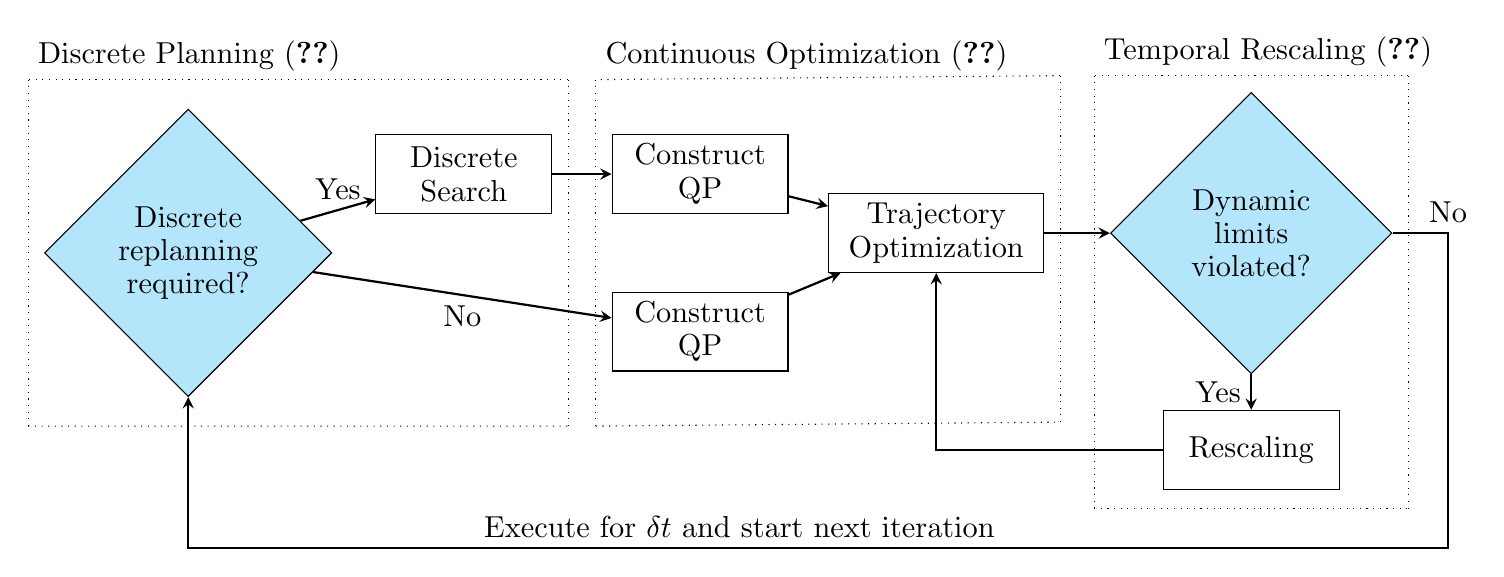
\begin{tikzpicture}[node distance = 2cm]
    \node (discrete) [decision, text width=2cm] {Discrete replanning required?};
    \node (discretesearch) [process, right of=discrete, xshift=1.5cm, yshift = 1cm, text width = 2cm] {Discrete Search};
    \node (discobjbuild) [process, right of=discretesearch, xshift = 1cm, text width = 2cm] {Construct QP};
    \node (contobjbuild) [process, below of=discobjbuild, text width = 2cm] {Construct QP};
    \node (trajopt) [process, right of=discobjbuild, yshift = -0.75cm, xshift = 1cm, text width = 2.5cm] {Trajectory Optimization};
    \node (dynamiclimits) [decision, right of=trajopt, xshift = 2.0cm, text width = 2cm] {Dynamic limits violated?};
    \node (rescale) [process, below of = dynamiclimits, text width = 2cm, yshift = -0.75cm] {Rescaling};

    \coordinate[above=2cm of discrete.west, xshift=-0.2cm, yshift=0.2cm] (c1);
    \coordinate[below=2cm of discrete.west, xshift=-0.2cm, yshift=-0.2cm] (c2);
    \coordinate[above=2cm of discretesearch.east, xshift = 0.2cm, yshift=-0.8cm] (c3);
    \coordinate[below=2cm of discretesearch.east, xshift = 0.2cm, yshift = -1.2cm] (c4);
    
    \coordinate[above=2cm of discobjbuild.west, xshift=-0.2cm, yshift=-0.8cm] (c5);
    \coordinate[below=2cm of discobjbuild.west, xshift=-0.2cm, yshift = -1.2cm] (c6);
    \coordinate[above=2cm of trajopt.east, xshift = 0.2cm] (c7);
    \coordinate[below=2cm of trajopt.east, xshift = 0.2cm, yshift=-0.4cm] (c8);
    
    \coordinate[above=2cm of dynamiclimits.west, xshift=-0.2cm] (c9);
    \coordinate[below=2cm of dynamiclimits.west, xshift=-0.2cm, yshift = -1.5cm] (c10);
    \coordinate[above=2cm of dynamiclimits.east, xshift = 0.2cm] (c11);
    \coordinate[below=2cm of dynamiclimits.east, xshift = 0.2cm, yshift = -1.5cm] (c12);
    
    \draw [arrow] (discrete) -- node[anchor=south] {Yes} (discretesearch);
    \draw [arrow] (discrete) -- node[anchor=north] {No} (contobjbuild);
    \draw [arrow] (discretesearch) -- (discobjbuild);
    \draw [arrow] (discobjbuild) -- (trajopt);
    \draw [arrow] (contobjbuild) -- (trajopt);
    \draw [arrow] (trajopt) -- (dynamiclimits);
    \draw [arrow] (dynamiclimits) -- ++(2.5,0) node[anchor=south] {No} -- ++(0,-4) --  ++(-5,0) -- ++(-4,0) node[anchor=south] {Execute for $\delta t$ and start next iteration} -|   (discrete);
    \draw [arrow] (dynamiclimits) -- node[anchor=east] {Yes} (rescale);
    \draw [arrow] (rescale) -| (trajopt);
    
    \node[right = 0cm of c1, yshift=0.3cm] {Discrete Planning (\ref{discretePlanning})};
    \node[right = 0cm of c5, yshift=0.3cm] {Continuous Optimization (\ref{continuousOptimization})};
    \node[right = 0cm of c9, yshift=0.3cm] {Temporal Rescaling (\ref{temporalRescaling})};
    
    \draw [dotted] (c1) -- (c2);
    \draw [dotted] (c2) -- (c4);
    \draw [dotted] (c4) -- (c3);
    \draw [dotted] (c3) -- (c1);
    
    \draw [dotted] (c5) -- (c6);
    \draw [dotted] (c6) -- (c8);
    \draw [dotted] (c8) -- (c7);
    \draw [dotted] (c7) -- (c5);
    
    
    \draw [dotted] (c9) -- (c10);
    \draw [dotted] (c10) -- (c12);
    \draw [dotted] (c12) -- (c11);
    \draw [dotted] (c11) -- (c9);
\end{tikzpicture}
}
\caption{Overview of the replanning pipeline.
}
\label{fig:flowchart}
\end{figure}

\subsection{Discrete Planning} \label{discretePlanning}
Robot $i$ executes discrete planning if any of the following conditions are true, where $\psi=K\delta t$ is the current time:
\begin{enumerate}
    \item The original trajectory is not collision-free for the desired time horizon $\tau$, i.e., $\exists t\in [\psi,\psi+\tau] : R(\vo_i(t)) \cap \cO_i \neq \emptyset$,
    \item The first piece of the previously planned trajectory is outside the robot's buffered Voronoi cell, i.e., $\exists t\in [0, T^{K-1}_{i,1}] : \vf^{K-1}_{i,1}(t) \not\in \cV_i$, or
    \item The previously planned trajectory is not collision-free for the desired time horizon $\tau$, i.e., $\exists t\in [0,\tau] :  R(\vf^{K-1}_i(t)) \cap \cO_i \neq \emptyset$.
\end{enumerate}
The first condition handles cases where previously unknown obstacles block the pre-planned path of a robot. The second condition handles cases where previously unknown robots appear and cases where robots are close and moving towards each other. The third condition handles dynamic obstacles, and  also infeasibilities and numerical issues that resulted in a trajectory with collisions in the previous iteration. 
Sections~\ref{theoreticalGuarantees} and Section~\ref{simulationSection} detail reasons for infeasibilities and  numerical issues, respectively.

Discrete planning uses a dynamic receding horizon approach. First, we find the earliest time $\tau'\in [\min(\tau, T_i-\psi), T_i-\psi]$ where the original trajectory is collision-free at time $\psi + \tau'$ with respect to both obstacles and other robots.
Second, we use a discrete graph search to find a path from the robot's current location to $\vo_i(\psi+\tau')$ that avoids both static obstacles and other robots.
If $\tau'$ does not exist or no solution path exists, we skip the discrete planning stage and construct the QP as if discrete planning was not required.
Third, we use the first $l$ segments of the discrete path to uniformly place the new estimated control points on top of those segments.
In case the discrete path has fewer than $l$ segments, the last discrete segment is shared between multiple B\'ezier curves.
Finally, we adjust $T_{i,j}^K$ relative to the segment lengths and scale by $\tau'$, such that we would arrive at time $\psi+\tau'$ at $\vo_i(\psi+\tau')$ if we followed the discrete path with constant speed.
To guarantee collision-free operation, we ensure that $T_{i,1}^K\geq \delta t$ in any case.

An example is shown in Fig.~\ref{fig:swap2_2} (a), with parameters $l=4$ and $d=7$.
Discrete planning is executed because the original trajectory (green dashed line) passes through an obstacle.
We find the earliest time $\tau'$ such that $R(\vo_g(\psi+\tau'))$ does not intersect with the obstacle and the blue robot where $g$ is the green robot.
The discrete planner is then used to find a path  (green dotted line) that avoids both the static obstacle and the other (blue) robot, with a total of six path segments.
The first four segments ($l=4$) are used to place new guesses of B\'ezier control points (blue, green, red, and cyan circles).
Notice that since $d=7$, each curve has eight control points, while some of the points are overlapping.
The duration $T^{K}_{i,j}$ for each B\'ezier curve is adjusted linearly according to its segment length; for example, the duration of the segment with the red control points ($T_{i,3}^K$) is approximately twice as long as the duration of the segment with the green control points ($T_{i,2}^K$).

\begin{figure}
\centering
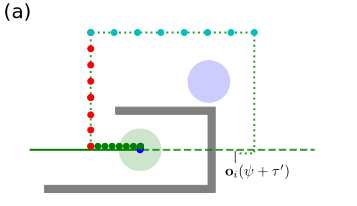
\includegraphics[width=0.49\textwidth]{images/swap2_discrete.pdf}
\hfill
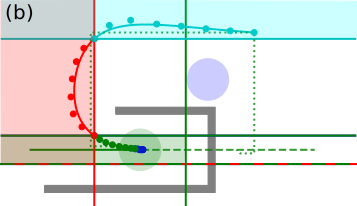
\includegraphics[width=0.49\textwidth]{images/swap2_cont_red.pdf}
\caption{
Example at $t=\SI{3.9}{s}$.
(a) Discrete path around an obstacle and other robot back to the original trajectory.
(b) Continuous trajectory split into four pieces and respective hyperspaces.
}
\label{fig:swap2_2}
\end{figure}

\subsection{Continuous Optimization}\label{continuousOptimization}
We compute a new trajectory by formulating a quadratic program where the decision variables are the concatenated control points of the pieces.
The parameters $d$ and $l$ of the pieces (see Section~\ref{bezierCurves}) are provided by the user.
If discrete planning is not performed, initial guesses of the decision variables are copied from the previous iteration, and the durations $T^{K}_{i,j}$ are set uniformly to $\frac{\min(\tau,T_i-\psi)}{l}$.
If discrete planning is performed, initial variables and durations are calculated from the discrete path as explained in Section~\ref{discretePlanning}.
The objective that we minimize is defined 
\begin{align}
    \sum_{e=1}^{\cE} \lambda_e\int_{0}^{T^K_i} \left\|\frac{d^e\vf^{K}_i(t)}{dt^e}\right\|^2dt + \sum_{j=1}^{l} \theta_j \left\|\vP^{K}_{i,j,d} - \vchi_{j}\right\|^2, \label{costFunction}
\end{align}
where $\vchi_j$ is the point  where we want piece $j$ to end.
The first term of the objective minimizes the energy along the trajectory, and is the combination of integrated squared derivatives up to user provided degree $\cE$ with weights $\lambda_e$ \cite{crazyplanning-ieeetro,richterISRR}.
The second term of the objective penalizes deviation from the given end points for each piece of the trajectory with different weights $\theta_j$.
In case discrete planning is performed, we attempt to get to the position of the last guessed control point, i.e., we set $\theta_l$ to a positive value, enforcing $\vP^K_{i,l,d} = \vchi_l$, and $\theta_j = 0,\,\forall j < l$.
If discrete planning is not performed, we attempt to stay as close as possible to the original trajectory, i.e.,  we set $\theta_1 = 0$, and $\theta_j, \forall j \geq 2$ to positive values (increasing with $j$) and $\vchi_j = \vo_i(\psi + \sum_{u=1}^j T^{K}_{i,u})$.
The matrix $H$ (see Section~\ref{trajectoryOptimization}) for the first term of our objective can be constructed as in our previous work~\cite{crazyplanning-ieeetro}.
The second term is a quadratic function of the control points; hence it is straightforward to construct the $H$ matrix and the $\vg$ vector.

For robot-to-robot collision avoidance, the buffered Voronoi hyperplanes are computed according to \eqref{voronoiAlphaBeta} and $m-1$ hyperspace constraints are added for the first piece.
These constraints ensure that the first piece stays inside $\cV_i$ because of the convexity of $\cV_i$ and the convex hull property of B\'ezier curves.
As long as $T^{K}_{i,1} \geq \delta t$ and all other robots stay inside their Voronoi cells up to time $\delta t$, we can be sure that no robot-to-robot collision will occur up to time $\delta t$.

For robot-to-obstacle collision avoidance we compute separating hyperplanes between convex obstacles $\cO_i$ for each curve piece $j$.
Let $M_j^b$ be the hyperplane that seperates the initially guessed control points of the $j\th$ piece from the $b\th$ convex obstacle obtained from $\cO_i$ (these can be computed, e.g., using support vector machines~\cite{SVM}).
We shift each hyperplane towards its obstacle and than shift it back using the radius $r_s$ to account for the physical extent of the robot.
We add hyperspace constraints as before, requiring control points of the $j\th$ piece in the non-occupied side of each hyperplane $M_j^b$.
These constraints ensure that no robot-to-obstacle collision will occur up to time $\tau'$.
In case discrete planning was executed, we additionally treat other robots as static obstacles.
Fig.~\ref{fig:swap2_2}(b) shows the effective set of hyperspaces for our example.

Moreover, we add continuity constraints that enforce the continuity requirements between pieces and initial point constraints that enforce continuity requirements between iterations.

All constraints are linear and matrix $A$ and its bounds can be constructed as in Section~\ref{trajectoryOptimization}.
The number of decision variables in our QP is $l(d+1)n$.
Let $\uptheta'$ describe the number of considered static obstacles, i.e., $\uptheta'$ is equal to $\uptheta + (m-1)$ if discrete planning was performed and $\uptheta$ otherwise.
We add $(m-1)(d+1) + \uptheta' l(d+1) + (c+1)nl$ linear constraints, where the terms refer to the Voronoi hyperspace, obstacle hyperspace, and continuity constraints, respectively.
For our example in Fig.~\ref{fig:swap2_2}, we have $n=2$, $m=2$, $d=7$, $l=4$, and $c=2$. Thus, we have 64 decision variables and $8 + 128 + 24 = 160$ linear constraints.

\subsection{Temporal Rescaling}  \label{temporalRescaling}
Since we use fixed durations of the pieces and do not account for the dynamic limits of the robot during optimization, the resulting trajectory may violate the dynamic limits of the robot.
After trajectory optimization, we calculate the maximum magnitudes $\Gamma_k$ of the $k\th$ derivatives of the curve, and check if there exists a $k$ such that $\Gamma_k > \gamma_k$, where $\gamma_k$ is the dynamic limit of the robot in the $k\th$ derivation degree.
If that is the case, we uniformly scale the piece durations $T^K_{i,j}$, and re-run the trajectory optimization with the same exact constraints using the previous result as the initial guess.
If the dynamic limits are not violated, no temporal rescaling is needed and the trajectory is feasible.

\subsection{Theoretical Guarantees} \label{theoreticalGuarantees}
For robot-to-robot collision avoidance our approach uses buffered Voronoi cells which has the following theoretical guarantee:
if robots start in a collision-free configuration (that is, $\|\vp_i - \vp_j\| \geq 2r_s, \forall i\neq j$), then all future configurations are collision-free.
However, this guarantee has only been proven for the case of synchronous robot execution, if robots have first-order integrator dynamics ($c=0$), and if they execute their trajectories perfectly~\cite{bufferedVoronoiCells}.
The QP in our formulation has additional constraints that can cause it to be infeasible. However, in this case, we can simply fallback to the QP formulation of the BVC approach, thus retain the same theoretical guarantee.

Formal guarantees under arbitrary disturbances and higher order dynamics cannot be provided.
In fact, our QP can fail if it is not feasible to satisfy all safety and continuity constraints under the given dynamic limits.
However, our empirical evaluation presented in Section~\ref{simulationSection} shows that the QP rarely fails and even if it does, the robots do not collide with each other and the obstacles since the QP becomes feasible in the following iterations.
In addition, our QP formulation allows us to easily detect failure cases because we model all safety-critical parts as hard constraints.

Similar to other work, there are no formal liveness guarantees and there might be deadlocks~\cite{bufferedVoronoiCells}.
Nevertheless, our approach works in practice for robots with higher-order dynamics, if robot execution is asynchronous, or trajectories are not executed perfectly.


\section{Evaluation} \label{evaluationSection}
We implement our approach in C\texttt{++}.
We use an occupancy grid as the environment representation, because previous work has shown that such data structures can be updated in real-time on robots that are equipped with a LIDAR sensor or an RGB-D camera.
In particular, OctoMap~\cite{octomap} is an octree-based 3D occupancy grid that can be run on unmanned aerial vehicles with at least \SI{4}{Hz} update rate~\cite{replanning-eth}.
OctoMaps are memory efficient, but update operations can show high execution time variance.
For local replanning, occupancy grids using ring buffers as data structures have been shown to achieve near constant execution time~\cite{replanning-usenko}.
Our implementation uses a simple pre-initialized 2D occupancy grid.

We use the CVXGEN-package~\cite{cvxgen} to generate small QPs to find separating hyperplanes between control points and obstacles.
We test with qpOASES~\cite{qpOASES} and OSQP~\cite{osqp} as QP solvers; both are open source and have been shown to work well in model predictive control scenarios. 

A supplemental video containing some of our simulations and physical experiments is available at \url{https://youtu.be/LbWRvLfdwTA}.

\subsection{Simulation}\label{simulationSection}
We test our algorithm in a simulation running on a laptop computer (i7-4700MQ \SI{2.4}{GHz}, \SI{16}{GB}) with Ubuntu 16.04 as the operating system.

In the first set of experiments, we test the scalability of our method in terms of the number of pieces $l$ we plan for, the number of occupied cells $\uptheta$ in the occupancy grid and the number of robots $m$.
Our results are summarized in Tables~\ref{tab:curveCountScalability}, \ref{tab:obstacleCountScalability} and \ref{tab:robotCountScalability}, where $t_{\text{avg}}$ is the average time that qpOASES takes per iteration.
Our algorithm scales well with the number of robots.
In terms of number of curves, our algorithm has almost the same performance up to $l=10$. For the simulations and physical experiments we did, we never needed more than $l=4$.
The bottleneck of our algorithm is the number of occupied cells in the occupancy grid. However, as it can be seen in Table~\ref{tab:obstacleCountScalability}, our algorithm still has real-time capability when considering hundreds of occupied cells, assuming a \SI{10}{Hz} execution.
When we use OSQP instead of qpOASES, our implementation takes significantly more time if we consider many obstacles.
For example, when we do experiment $7$ using OSQP, it takes \SI{297}{ms} on average.

\begin{table}[!htb]% 
\begin{minipage}{.3\textwidth}
    \centering
    \begin{tabular}{|l|c|c|c|c|r|}
        \hline
         \#&$l$&$\uptheta$ &$m$&$t_{\text{avg}}\,[\si{ms}]$  \\ \hline
         1 & $4$ & $0$ & $4$ & $10$\\ \hline
         2 & $8$ & $0$ & $4$ & $15$\\ \hline
         3 & $10$ & $0$ & $4$ & $13$ \\ \hline
         4 & $12$ & $0$ & $4$ & $27$ \\ \hline
         5 & $16$ & $0$ & $4$ & $107$ \\ \hline
         \multicolumn{5}{c}{}\\
    \end{tabular}
    \caption{Runtime with varying curve count $l$.}
    \label{tab:curveCountScalability}
\end{minipage}
\hfill
\begin{minipage}{.3\textwidth}
    \centering
    \begin{tabular}{|l|c|c|c|c|r|}
        \hline
         \#&$l$&$\uptheta$ &$m$&$t_{\text{avg}}\,[\si{ms}]$  \\ \hline
         6 & $4$ & $4$ & $4$ & $9$ \\ \hline
         7 & $4$ & $62$ & $4$ & $28$ \\ \hline
         8 & $4$ & $196$ & $4$ & $47$  \\ \hline
         9 & $4$ & $213$ & $4$ & $69$  \\ \hline
         10 & $4$ & $1250$ & $4$ & $253$  \\ \hline
         \multicolumn{5}{c}{}\\
    \end{tabular}
    \caption{Runtime with varying occupied cells $\uptheta$.}
    \label{tab:obstacleCountScalability}
\end{minipage}
\hfill
\begin{minipage}{.3\textwidth}
    \centering
    \begin{tabular}{|l|c|c|c|c|r|}
        \hline
         \#&$l$&$\uptheta$ &$m$&$t_{\text{avg}}\,[\si{ms}]$  \\ \hline
         11 & $4$ & $5$ & $4$ &$9$\\ \hline
         12 & $4$ & $5$ & $8$ & $10$ \\ \hline
         13 & $4$ & $5$ & $16$ & $13$ \\ \hline
         14 & $4$ & $5$ & $32$ & $15$  \\ \hline
         15 & $4$ & $5$ & $64$ & $14$  \\ \hline
         \multicolumn{5}{c}{}\\
    \end{tabular}
    \caption{Runtime with varying robot count $m$.}
    \label{tab:robotCountScalability}
\end{minipage}
\vspace{-10mm}
\end{table}


\begin{table}
    \centering
    \begin{tabular}{ |c|  c|c  | c| c| c| c| c| c| c|}
      \cline{4-10}
       \multicolumn{3}{c|}{} & \multicolumn{2}{c| }{ORCA} & \multicolumn{2}{c| }{DS+ORCA} & \multicolumn{3}{c|}{Our Method}\\ \hline
      \# & $m$ &  $\uptheta$ &  $t_{\text{avg}}\,[\si{ms}]$  & $s$ & $t_{\text{avg}}\,[\si{ms}]$  & $s$ & $t_{\text{avg}}\,[\si{ms}]$  & $s$ & QP failures [\%]\\ \hline
      $16$ & $2$ & $4$  & $<1$  & $0$ & $<1$  & $2$ & $7$  & $2$ & $0.00$\\ \hline
      $17$ & $4$ & $12$  & $<1$  & $0$ & $<1$  & $4$ & $10$  & $4$ & $0.30$\\ \hline
      $18$ & $8$ & $30$  & $<1$  & $4$ & $<1$  & $8$ & $13$  & $8$ & $0.00$\\ \hline
      $19$ & $16$ & $9$ & $<1$  & $13$ & $<1$  & $16$ & $12$  & $16$ & $0.08$\\ \hline
      $20$ & $32$ & $30$ & $<1$ & $23$ & $<1$ & $32$ & $16$ & $32$ & $0.09 $\\ \hline
      \multicolumn{9}{c}{} \\
    \end{tabular}
    \caption{Comparison of our method, ORCA, and DS+ORCA with respect to average computation time ($t_{\text{avg}}$), the number of robots that reach  their destinations ($s$), and the percentage of time that our QP fails.
    }
    \label{tab:rvo2Comparison}
\end{table}

We also compare our method to two ORCA variants in the second set of experiments.
In the first ORCA variant, we use the RVO2 library~\cite{orca} and set the preferred velocities at time $\psi$ to $\vo_i'(\psi)$ if $\vp_i\approx \vo_i(\psi)$ or to $\frac{\vo_i(\psi) - \vp_i}{\delta t}$ otherwise.
In the second ORCA variant, we combine ORCA and our discrete planning method with a dynamic receding horizon approach (denoted as DS+ORCA). We demonstrate that this variant resolves deadlocks better than the first variant.
For our method we use $\delta t = \SI{0.1}{s}$, $l=4$, and $d=7$ and for the ORCA variants we use $\delta t = \SI{0.01}{s}$.
The results are summarized in Table~\ref{tab:rvo2Comparison}.
All robots using our method or DS+ORCA reach their destinations, while robots using ORCA can easily get stuck around obstacles.
Our method takes more time in computation compared to the ORCA variants, but produces smooth curves up to a user-defined smoothness.
We use $c=2$ in our experiments meaning that the generated trajectories are continuous in position, velocity, and acceleration.
The ORCA variants, on the other hand, provide smoothness guarantees up to $c=0$ only, i.e., velocities can jump between iterations.
Furthermore, the ORCA variants must sense the other robots' velocities and positions while our approach relies on positions only.

We also report the percentage of time our QP fails, which happens no more than $\SI{0.3}{\percent}$ of the time. Notice that even if our QP fails, robots do not collide with each other and the obstacles, because the QP becomes feasible in the following iteration after $\SI{100}{ms}$. There are two reasons for QP failures: infeasibilities, which are explained in Section~\ref{theoreticalGuarantees}, and numerical issues. The numerical issues stem from separating hyperplane calculations between robots and obstacles. We use hard-margin SVMs to calculate separating hyperplanes. When robots get too close to obstacles, small epsilon values in SVM optimization may result in invalid hyperplanes, and hence QP fails.
The original trajectories and the occupancy grids in some experiments are shown in Fig.~\ref{fig:examples} and the supplemental video contains selected simulations.

% experiments 17, 19 and physical
\begin{figure}
\centering
\includegraphics[width=0.32\textwidth]{images/ex_17.pdf}
\hfill
\includegraphics[width=0.32\textwidth]{images/ex_19.pdf}
\hfill
\includegraphics[width=0.33\textwidth]{images/physical.pdf}
\caption{
The original trajectories and the occupancy grids in the simulation experiments 17 (a), 19 (b), and the physical experiment (c).
}
\label{fig:examples}
\end{figure}

\subsection{Physical Robots}
We implement our approach on six differential drive robots (iRobot Create2) that are equipped with one of ODROID C1+ or ODROID XU4 single-board computers.
Those computers run Ubuntu 16.04 with ROS Kinetic, but C1+ has very limited computation capabilities (ARM Cortex-A5, max. \SI{10}{W}).
The robots are arranged in a circle (\SI{2}{m} radius) and are tasked with swapping sides (Fig.~\ref{fig:examples}c).
We plan the original trajectories with one static obstacle using a centralized planner~\cite{crazyplanning-heterogeneous}.
Each robot receives the position information of all other robots using a motion capture system.
A trajectory tracking controller and our algorithm run on-board at a frequency of \SI{10}{Hz}.

We conduct several experiments and add an additional obstacle, change the robots initial position, disturb the robots during run-time, or artificially stop one of the robots.
In all cases robots successfully avoid collisions and in many cases they reach their final destination within the originally planned durations.
We also saw a few cases where robots got into a deadlock, which we attribute to the fact that the robots, unlike the simulation, cannot execute very low velocity commands.
The supplemental video includes recordings of our experiment.


\section{Conclusion}
We present a method for robust trajectory execution that takes pre-planned trajectories as input and compensates for a variety of dynamic changes, including imperfect motion execution, newly appearing obstacles, robots breaking down, or external disturbances.
Our approach does not require communication between the robots.
We use a novel planning strategy employing both discrete planning and trajectory optimization with a dynamic receding horizon approach.
We demonstrate in simulation and on physical robots that we can generate smooth trajectories in real-time, while avoiding deadlocks successfully. In comparison, ORCA neither generates smooth trajectories nor avoids deadlocks in our test cases.

In future work we would like to conduct additional experiments with robots using on-board perception and flying robots; handle dynamic obstacles; and consider communication between robots to improve their plans. We also would like to actively address numerical issues and QP infeasibilities.

\vfill

\pagebreak

%
% ---- Bibliography ----
%
\bibliographystyle{spmpsci}
\bibliography{bibliography}

\end{document}
